\documentclass{UoNMCHA}
\usepackage[authoryear]{natbib}
\usepackage{array,booktabs} % For nice tables
\usepackage{amsmath,amsfonts,amssymb} % For nice maths
\usepackage{color,mathtools}
\usepackage{enumerate,tensor}
\usepackage{listings}
\usepackage{subfig}
\usepackage{multicol}
\usepackage{hyperref}
\usepackage{float}
\usepackage[parfill]{parskip}   % For replacing paragraph indenting with a newline instead

% Number equations per section
\numberwithin{equation}{section}

\hypersetup{
%    bookmarks=true,         % show bookmarks bar?
%    unicode=false,          % non-Latin characters in AcrobatÕs bookmarks
%    pdftoolbar=true,        % show AcrobatÕs toolbar?
%    pdfmenubar=true,        % show AcrobatÕs menu?
%    pdffitwindow=false,     % window fit to page when opened
%    pdfstartview={FitH},    % fits the width of the page to the window
%    pdftitle={My title},    % title
%    pdfauthor={Author},     % author
%    pdfsubject={Subject},   % subject of the document
%    pdfcreator={Creator},   % creator of the document
%    pdfproducer={Producer}, % producer of the document
%    pdfkeywords={keyword1} {key2} {key3}, % list of keywords
%    pdfnewwindow=true,      % links in new window
    colorlinks=true,       % false: boxed links; true: colored links
    linkcolor=blue,          % color of internal links
    citecolor=blue,        % color of links to bibliography
%    filecolor=magenta,      % color of file links
    urlcolor=blue           % color of external links
}

\definecolor{MATLABKeyword}{rgb}{0,0,1}
\definecolor{MATLABComment}{rgb}{0.1328125,0.54296875,0.1328125}
\definecolor{MATLABString}{rgb}{0.625,0.125,0.9375}

\lstset{language=Matlab,
    basicstyle=\small\ttfamily,
    keywordstyle=\color{MATLABKeyword},
    %identifierstyle=,
    commentstyle=\color{MATLABComment},
    stringstyle=\color{MATLABString},
    numberstyle=\tiny,
    %numbers=left,
    basewidth=0.5em}

\firstpage{1}    % Set page number for first page
\UoNMCHAreportNo{FYP} %Report number
\UoNMCHAyear{2019}   % Year\\
\shorttitle{Vision-Based Control of an Industrial Robot Arm} %For odd pages
%%%%%%%%%%%%%%%%%%%%%%%%%%%%%%%%%%%%%%%%%%%%%%%%%%%%
\begin{document}
\title{Vision-Based Control of Industrial Robot Arm \\ \ \\
{\small 31/10/2019}}
\author[UoNMCHA]{Muhammad Hasham Khan}
\address[UoNMCHA]{
Student of Mechatronics Engineering,\\
The University of Newcastle, Callaghan, NSW 2308, AUSTRALIA \\
Student Number: 3256011 \\
E-mail: \href{mailto:c3256011@uon.edu.au}{\textsf{c3256011@uon.edu.au}}}
%%%%%%%%%%%%%%%%%%%%%%%%%%%%%%%%%%%
\maketitle
\onecolumn

\vspace{-5mm}
\section*{Executive summary}
\vspace{-3mm}
 
%\begin{itemize}
%    \item Defines the intention of the report.
%    \item Places the report in context so the reader knows why it is important to read it.
%    \item Why is it important?
%    \item What problem is addressed?
%    \item Briefly states the results
%    \item Briefly presents the implications and recommendations
%\end{itemize}
%Executive summaries can take from a couple of paragraphs to a couple of pages.\\

This project aims to demonstrate a visual servoing system for an industrial robotic manipulator and its practical use. Vision based control is a growing field in the robotic world being used to guide autonomous vehicles and control industrial manipulators. This project explores the vision based control approach to develop a control scheme that uses a camera to guide the end effector of the ABB robot arm and an algorithm to classify objects.\\

 This task involves developing a control scheme for visual servoing, training an object classifier, designing a minimal path planner, demonstrating the manipulator in simulation and operating the robot to reach a desired position for the end effector. The simulation and hardware demonstration task will be split between part A and part B.\\
 
  Future work for this project involves performing a hardware demonstration using simulation environments and experiments with the ABB robot. 

%%%%%%%%%%%%%%
\vspace{-2mm}
\section*{Acknowledgements}
\vspace{-3mm}
You may like to say thank you to someone that helped you with your project.
\newpage
\tableofcontents
\newpage
%%%%%%%%%%%%%%%%%%%%%%%%%%%%%%%
\section{Introduction}
%To organise your introduction section you can use the following structure:
%\begin{itemize}
%    \item \textbf{Position}: Show there is a problem and that it is important to solve it.
    
   \subsection{Background}
   Robotic manipulators are very useful since they can perform precise, repetitive and dangerous tasks that humans cannot because of their speed, accuracy and reliability. Due to their benefits, they are used to automate tasks such as welding [CITE ME], painting vehicles [CITE ME] and even harvesting crops CITE ME[]\\ 
      
   Automation of robotic manipulatos has been done in manufacturing, painting cars, gimbals etc using different kinds of sensors such as IMU's and laser range finders [cite me]\\
   
   A very useful technique is using cameras to performs this control. It uses less sensors, can be more economical, can use sensor fusion to combine multiple cameras. This is especially useful when the robotic manipulator is not in a predefined environment. An example is the robot arm on the mars curiosity rover [cite me] \\
   
   This technique is known as visual servoing, and it has two commonly used techniques. \\
   One is to use a fixed point camera that views the object in space while another is a camera attached to the end effector.\\
    here are the benefits of each:\\
    - eye in hand results in closed loop control while fixed camera is an open loop system\\
    
    
    
    
    \subsection{Problem statement}
%    \item \textbf{Problem}: Describe the specifics of the problem you are trying to address
    
   The goal of this project is to use an end effector camera to perform a common automation task used in industry; to sort and pick and place predifined objects using visual control using a industrial robotic manipulator. \\
   
   exampes of such a task are harvesting robots, car painting robots in factories and the mars rover arm\\
       
    ASSUMPTIONS\\
    This task involves sorting predefined objects on a known workspace into known locations. The predefined objects need to be of uniform shape, be visually differentiable and be easily movable by the arm \\
    The location bins may be a marked location on the workspace\\
    The workspace itself will be a flat table surface free of obstructions and with suitable lighting 
    
    
    
    - To perform this task, we need to:\\
    	1 Classify objects to be sorted\\
    	2 Locate objects to be sorted using a camera\\
    	3 Generate a trajectory to sort items\\
    	4 Control a robotic manipulator to reach desired end effector pose's // follow a path\\
    	5 Design a visual servoing system to control the robot  
    	
  	
%    \item \textbf{Proposal}: Discuss how you are going to address this problem. Use the literature to back-up your approach to the problem, or to highlight that what you are doing has not been done before
    \subsection{Literature Review}
    
    - 1: classifying objects in an image has been done using "examples".\\
    can classify an image or you can classify the location the object is in the image.\\
     there have been many recent advances in the field, e.g. alexnet popularising the cnn architecture and the subsequent boost in the use of GPU's.\\
     Talk about RCNN, fast RCNN and faster RCNN and then that vs SSD vs YOLO vs RESNET etc.\\
     The decision to use tensorflows open source libraries vs matlab.\\
     Ultimately, Faster RCNN was chosen as it provides the greatest accuracy at the cost of greater computing time. This was not an issue for this project as speeds will be limited \\
    
    - 2: Locating objects is done using line detection and feature extraction. These features can then be manipulated to find the location of the object relative to the end effector position or used directly to control the movement of the arm.\\
    
    - 3: Items can be arbritarily placed on a work surface and the minimal path to each points needs to be generated. This can be seen as a subset of the travelling salesman problem, whereby each point can be seen as node that can only be visited once.\\
    The soluton can  then be used to generate a path as a series of discrete poses in the operation space for the end effector to follow.\\
    
    - 4: This component requires a simulation model of the robotic manipulator and forward and inverse kinematics to follow a desired trajectory. \\
    - 5: This component requires interfacing with the manipulator through a controller, interfacing with the camera and getting images and generating a control action. PBVS vs LBVS
    
    
%\end{itemize}
%Here you need to sell why what you are doing is important, and what benefits will it bring if you are successful and solve the problem? 

\subsection{Motivation}

the use of machine vision systems for control automisation is part of modern control structures. \\
this project aims to demonstrate and implement these techniques on a real platform. wants to integrate vision control with industrial robot. to select classify and manipulate objects.\\
This is a benchmark but these techniques can be implemented/adapted to other tasks more relevant to industry.\\   
integration of vision within robotics was not part of my degree and was useful to learn  


%The rest of the report is organised as follows. Section~\ref{sec:Core Section} describes items related to the core content. Section~\ref{sec:Conclusion} concludes the report. Appendix~\ref{app:Table} shows an example of how to make a Table.
%%%%%%%%%%%%%%%%%%%%%%%%%%%%%%%
\newpage
\section{Robotic Manipulator Simulation}\label{sec:Core Section}


To perform a pick and place task, a suitable robotic manipulator was required. The ABB IRB 120 robotic manipulator was provided by the University of Newcastle to be used:
\subsection{ABB IRB 120}
- introduce the robot and its specifications\\
The IRB 120 is a 6DOF robotic manipulator commonly used in industry due to it's small size and high manuevarability. It can carry a payload of 3Kg at it's end effector, can reach 580mm horizontally from it's base and an end effector accuracy of 0.5mm. This makes it ideal for the desired pick and place task\\
- The anthropomorphic structure of the ABB robot arm mimics the functionality of a real human arm, albeit with one less degree of freedom.\\
- the desired end effector is not available and will be chosen or designed in part B. Such a system's design criterion and subsequent impacts with be further discussed in section XX\\
- To use the robotic arm, a simulation model was required 

\subsection{Modelling}

Modelling of the robot can be done as an open serial kinematic chain. This involves defining a co-ordinate system for each joint of the \\
The robot consists of 6 joints that can move freely about an axis, as shown in Figure~\ref{fig:Anthro}

\begin{figure}[ht]
	\begin{center}
		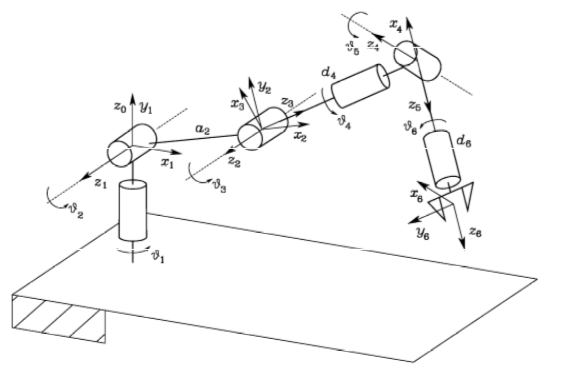
\includegraphics[width=.6\linewidth]{Figures/Anthroarm}
		\caption{an Anthropomorphic arm, from Siciliano}
		\label{fig:Anthro}
	\end{center}
\end{figure}

One can then perform co-ordinate transformations to define a subsequent joint in terms of a rotation about the prior joint.\\
The Denavit Hartenberg convention was used to simplify many of these transformations\\
It works by standardising revolutions and prismatic extensions to only occur about the z axis.

The Denavit hartenberg paramaters were used and found at https://robodk.com/Python-API-examples

\begin{table}[h]
	\centering
	\caption{Denavit Hartenberg parameters for ABB IRB 120}
	\begin{tabular}{l|llll}
		& \textbf{q} & \textbf{d} & \textbf{a} & \textbf{alpha}  \\ 
		\hline
		\textbf{Joint 1} & 0          & 0          & 290        & -pi/2           \\ 
		\hline
		\textbf{Joint 2} & -pi/2      & 270        & 0          & 0               \\ 
		\hline
		\textbf{Joint 3} & 0          & 70         & 0          & -pi/2           \\ 
		\hline
		\textbf{Joint 4} & 0          & 0          & 302        & pi/2            \\ 
		\hline
		\textbf{Joint 5} & pi/2       & 0          & 0          & -pi/2           \\ 
		\hline
		\textbf{Joint 6} & pi         & 0          & 72         & 0               \\
		\hline
	\end{tabular}
\end{table}\

The transformation matrix is composed using

\begin{equation}[h]
	\prescript{N-1}{}T_{N} = Rot(q) Trans(d) Rot(a) Trans(\alpha)
\end{equation} 

Which results in the following co-ordinate transformation matrix describing the current joint with respect to the previous\

\begin{equation*}
\mathbf{\prescript{n-1}{}T_{n}} =
\begin{bmatrix}
cos\theta_n & -sin\theta_ncos\alpha_n & sin\theta_ncos\alpha_n  & r_n cos\theta_n \\
sin\theta_n & cos\theta_ncos\alpha_n  & -cos\theta_nsin\alpha_n & r_n sin\theta_n \\
0           & sin\alpha_n	 		  & cos\alpha_n				& d_n\\
0 			& 0						  & 0						& 1
\end{bmatrix}.
\end{equation*}

\subsection{Forward Kinematics}
Using the parameters from Table 1, the following Transformation matrices were constructed:

\begin{equation*}
\mathbf{\prescript{0}{}A_{1}} =
\begin{bmatrix}
cosq_1 & -sinq_1 & 0  & 0 \\
sinq_1 & cosq_1  & 0  & 0 \\
0      & 0       & 0  & d_1\\
0 	   & 0	     & 0  & 1
\end{bmatrix}.
\end{equation*} \

\begin{equation*}
\mathbf{\prescript{1}{}A_{2}} =
\begin{bmatrix}
cosq_2 & 0 & -sinq_2  & 0 \\
sinq_2 & 0  & cosq_2  & 0 \\
0      & -1  & 0  & 0\\
0 	   & 0	 & 0  & 1
\end{bmatrix}.
\end{equation*}

\begin{equation*}
\mathbf{\prescript{2}{}A_{3}} =
\begin{bmatrix}
cosq_3 & -sinq_3 & 0  & a_3 cosq_3 \\
sinq_3 & cosq_3  & 0  & a_3 sinq_3 \\
0      & 0  & 1  & 0\\
0 	   & 0	 & 0  & 1
\end{bmatrix}.
\end{equation*}

\begin{equation*}
\mathbf{\prescript{3}{}A_{4}} =
\begin{bmatrix}
cosq_4 & 0 & -sinq_4  & a_4 cosq_4 \\
sinq_4 & 0  & cosq_4  & a_4 sinq_4 \\
0      & -1  & 0  & d_4\\
0 	   & 0	 & 0  & 1
\end{bmatrix}.
\end{equation*}

\begin{equation*}
\mathbf{\prescript{4}{}A_{5}} =
\begin{bmatrix}
cosq_5 & 0 & -sinq_5  & 0 \\
sinq_5 & 0  & -cosq_5  & 0 \\
0      & 1  & 0  & 0\\
0 	   & 0	 & 0  & 1
\end{bmatrix}.
\end{equation*}

\begin{equation*}
\mathbf{\prescript{5}{}A_{6}} =
\begin{bmatrix}
cosq_6 & 0 & -sinq_6  & 0 \\
sinq_6 & 0  & -cosq_6  & 0 \\
0      & -1  & 0  & d_6\\
0 	   & 0	 & 0  & 1
\end{bmatrix}.
\end{equation*}\

and a purely horizontal translation to get from the spherical wrist to the end effector
\begin{equation*}
\mathbf{\prescript{6}{}A_{ee}} =
\begin{bmatrix}
1 & 0 & 0  & 0 \\
0 & 1  & 0  & 0 \\
0      & 0  & 1  & d_ee\\
0 	   & 0	 & 0  & 1
\end{bmatrix}.
\end{equation*}\

To find the transformation matrix that that relates the origin to the location of the end effector, we can
multiply the transformation matrices as follows:\\

\begin{equation}
\mathbf{\prescript{0}{}T_{ee}} = \mathbf{\prescript{0}{}A_{1}}\mathbf{\prescript{1}{}A_{2}}\mathbf{\prescript{2}{}A_{3}}\mathbf{\prescript{3}{}A_{4}}\mathbf{\prescript{4}{}A_{5}}\mathbf{\prescript{5}{}A_{6}}\mathbf{\prescript{6}{}A_{ee}}
\end{equation} 

where the matrix is comprised of:\\

\begin{equation*}
\mathbf{\prescript{6}{}A_{ee}} =
\begin{bmatrix}
\mathbf{\prescript{0}{}R_{ee}} & \mathbf{\prescript{0}{}r_{ee}}   \\
0 & 1  \\
\end{bmatrix}.
\end{equation*}\

where $R^{0}_{ee}$ is:

\begin{equation*}
\mathbf{R^{0}_{ee}} =
\begin{bmatrix}
R_{11} & R_{12} & R_{13} \\
R_{21} & R_{22} & R_{23} \\
R_{31} & R_{32} & R_{33} \\
\end{bmatrix}.
\end{equation*}\

These equations were then used in matlab to create a simulation of the model to be used for verification and which would return the end effector pose. The translational component is simply the vector $\mathbf{\prescript{0}{}r_{ee}}$. \
 However, the rotational component is unintuitive when extracted as a rotation matrix. Therefore, it was converted to euler angles using:

\begin{equation*}
\mathbf{\Theta^{0}_{ee}} =
\begin{bmatrix}
\phi \\ \theta \\\psi 
\end{bmatrix}
= 
\begin{bmatrix}
atan2(R_{32} , R_{33}) \\
atan2(-R_{31} , \sqrt{R_{33}^{2} + R_{33}^{2}}) \\
atan2(R_{21} , R_{11}) 
\end{bmatrix}
\end{equation*}\

\begin{figure}[ht]
	\begin{center}
		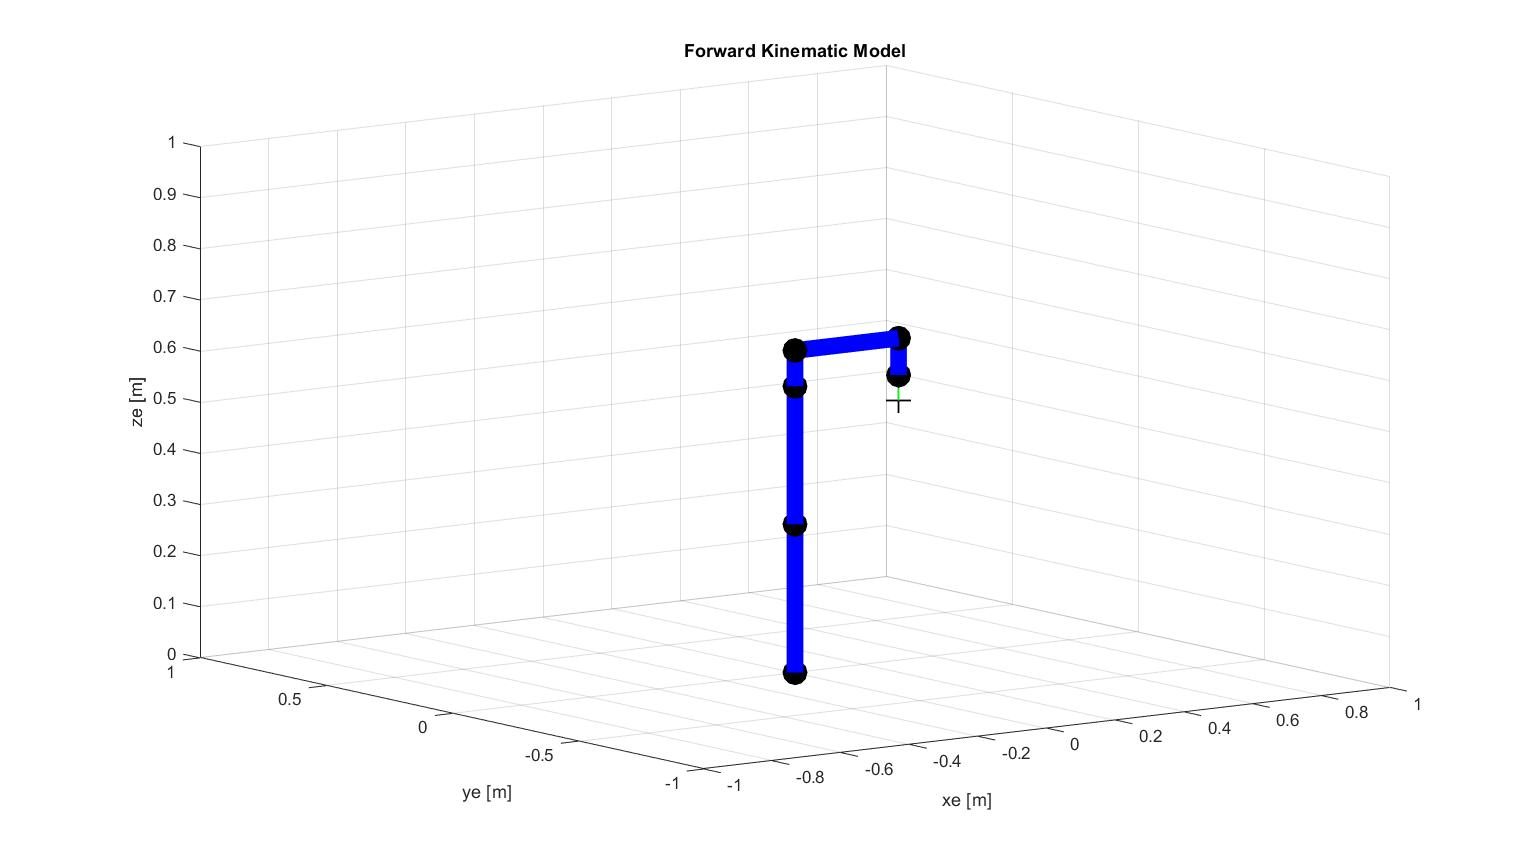
\includegraphics[width=.6\linewidth]{Figures/fkinmodel}
		\caption{Forward kinematic model simulation}
		\label{fig:fkmod}
	\end{center}
\end{figure}\

which was then verfied using RobotStudio to ensure the simulated pose of the end effector was consistent with the robot controllers software

\subsection{Inverse Kinematics}

Solving the Forward kinematic problem to find the joint angles required for a certain configuration is useful. However, tasks are performed in the cartesian space. Thus, a method is required to prescribe a end effector pose in the task space which will return the joint angles required in joint space. This problem is known as inverse kinematics.\\

A method to solve the inverse kinematic problem numerically requires the use of the Jacobian.\\

The Jacobian is defined as:\

\begin{equation*}
\mathbf{J} =
\begin{bmatrix}
J_{v} \\ J_{\omega}  
\end{bmatrix}
\end{equation*}\

where $J_{v}$ and $J_{\omega}$ relate to the linear and angular velocity of the joint in cartesian space to the rate of change of it's joint angles in joint space:\

\begin{equation*}
\begin{split}
\mathbf{v^{0}_{n}} = \mathbf{J_{v}}(q)\dot{q} \\
\mathbf{\omega^{0}_{n}} = \mathbf{J_{\omega}}(q)\dot{q} 
\end{split}
\end{equation*}\

The Jacobian of the ABB was computed using:\

\begin{equation*}
\mathbf{J} =
\begin{bmatrix}
J_{v} \\ J_{\omega}  
\end{bmatrix} = 
\begin{bmatrix}
R^{0}_{i-1} \begin{pmatrix}
0 \\0\\1 
\end{pmatrix}(r^0_n - d^0_{i-1})\\
 R^{0}_{i-1} \begin{pmatrix}
 0 \\0\\1 
 \end{pmatrix}  
\end{bmatrix}
\end{equation*}\

The Jacobian for the ABB is then constructed:

\begin{equation*}
\mathbf{J} =
\begin{bmatrix}
J_{v_1} & J_{v_2} & J_{v_3} & J_{v_4} & J_{v_5} & J_{v_6}  \\
 J_{\omega_1} & J_{\omega_2} & J_{\omega_3} & J_{\omega_4} & J_{\omega_5} & J_{\omega_6}  
\end{bmatrix}
\end{equation*}\

Thus, the geometric jacobian has been constructed. However, to have the ability to prescribe rates of change of angular velocity in roll, pitch and yaw rates, an analytical jacobian is required where:\

\begin{equation*}
\begin{split}
\mathbf{J_A} = \mathbf{T_A (\Theta^0_n)J} \\
\mathbf{T_A (\Theta^0_n)} =
\begin{bmatrix}
\mathbf{I} & \mathbf{0} \\
\mathbf{0} & \mathbf{E^{-1}(\Theta^0_n)} 
\end{bmatrix} \\
\mathbf{E (\Theta^0_n)} =
\begin{bmatrix}
1 & 0 & -sin\theta\\
0 & cos\phi & -sin\phi cos\theta\\
0 & -sin\phi & cos\phi cos\theta\\
\end{bmatrix}
\end{split}
\end{equation*}\

This anaytical jacobian can then be used to reach a desired pose $x_d$ from current pose $x_e$ where:

\begin{multicols}{2}
	\begin{equation*}
	\mathbf{x_e} =
	\begin{bmatrix}
	r^0_{n} \\
	\Theta^0_{n} 
	\end{bmatrix}
	\end{equation*}\break
	\begin{equation*}
	\mathbf{x_d} =
	\begin{bmatrix}
	r^{0 }_{n} \\
	\Theta^{0 }_{n} 
	\end{bmatrix}
	\end{equation*}\	
\end{multicols}

can be used to form an error function e\

\begin{equation*}
\mathbf{e = x_d - x_e} 
\end{equation*}\

Taking the derivate gives:\

\begin{equation*}
\mathbf{\dot{e} = \dot{x_d} - \dot{x_e} = \dot{x_d} - J_A(q)\dot{q}} 
\end{equation*}\

an

Leads to the following control structure:\

\begin{figure}[ht]
	\begin{center}
		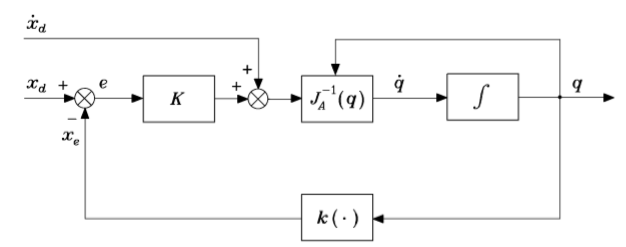
\includegraphics[width=.6\linewidth]{Figures/ode}
		\caption{Inverse kinematic model Control Scheme}
		\label{fig:ode}
	\end{center}
\end{figure}\

Which was simulated in Matlab and was used to follow a desired path, as shown:\

\begin{figure}[H]
	\begin{center}
		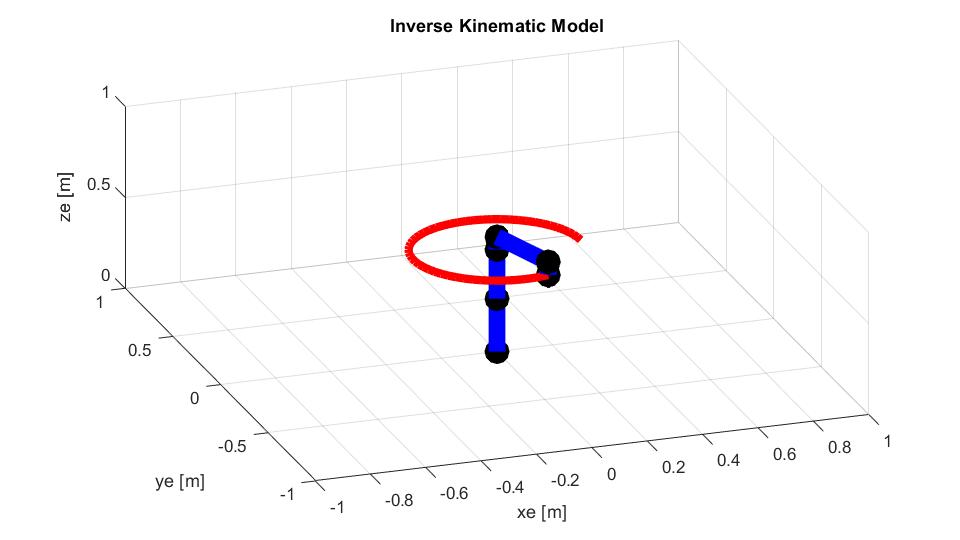
\includegraphics[width=.6\linewidth]{Figures/ikmodel}
		\caption{Inverse kinematic model Simulation}
		\label{fig:ikmodel}
	\end{center}
\end{figure}\

Thus, a simulation model of the ABB IRB 120 has been constructed which can follow a desired trajectory.\
The next section will now discuss the how the robot will be controlled to follow a trajectory such that it picks and places desired objects. 

%%%%%%%%%%%%%%%%%%%%%%%%%%
\newpage
\section{Object Classification}
What camera was used, how it was set up, how the training data was gathered, labelled and the accuracy validated
\subsection{Method}
- how the learning actually works in a faster rcnn, with the training set and the validation set used to minimise an error function which backpropogates through the layers, changing their weights\\
\subsection{Dataset Generation}
- initially the chameleon cmln-13s2c was to be used. However, specification were not suitable for the task.\\
- another camera will be used for the second half, in the meanwhile a rasberry pi camera is used
- took 200 images of each class in different environments with varying lighting conditions and backgrounds to ensure robustness\\
- also had negatives, which obscured the image in the form of glare and obstructed views
- used an open source software called LabelImg

\subsection{Training and Validation}
- training was performed on both matlab and tensorflow using inbuilt libraries\\
- comparison between faster rcnn vs ssd on this dataset \\
- faster rcnn was more accurate albeit slower, but that is fine as the robot will not be moving very fast. thus faster rcnn will be used in part B

\newpage
\section{Object Localisation}

How to perform image transforms and how to localise objects as a pose relative to the base of the robot or the end effector
\subsection{Image Jacobians}
- how an image jacobian works i.e. maps the location of a point on an image as pixels to the location of the point in cartesian co-ordinates\\
- we know the end effector and the camera and thus we can get the location of points of interest
- The jacobian and transformation for our system to get from camera to certain end points.\\
The desired points will be found using edge detection. This will produce unique quadrilaterals whose intersection points will be used as desired feature points.

\subsection{Simulation}
- This can shown using this example image, which is then transformed to give the desired feature points

\newpage
\section{Trajectory Generation}

Talk about travelling salesman problem and how it got solved and what constraints had to be used and how i fixed it and had it work for an arbritrary number of objects to be moved max 10
\subsection{travelling salesman problem}
- topological problem, can use a minimiser to find the optimal path 
- how to represent it mathematically and the constraints 
- how this was modified to use in our problem
\subsection{Simulation}
- examples of how the simulation worked which was used for validation and shows the desired trajectory 


\newpage
\section{Visual Servoing}

- this task involves using camera input and a desired trajectory to control the serial manipulator \\

- uses object classifier to classify each object\\
- This is used by the object localiser to determine its feature points and cartesian co-ordinates \\
- This is used by the trajectory generator to determine the optimal path \\
- follows the desired trajectory by controlling the robot arm using visual servoing. \\

\newpage
\section{Future Work}

What still needs to be done to get a hardware demonstration: 

- demonstrate visual servoing in simulation \\
- Configure RobotStudio and the ABB robot controller to receive serial commands from Matlab\\





\section{Conclusion}\label{sec:Conclusion}
%This is one of the most important parts of the report. In the conclusion section, you  should 
%\begin{itemize}
%\item briefly summarise the results,
%\item reflect on the work presented, 
%\item make recommendations,
%\item suggest future work or improvements.
%\end{itemize}

 %%%%%%%%%%%%%%%%%%%%%%%%%%%%%%%
\section{References and Citations}\label{sec:RefCite}
%To generate the bibliography look at the end of this document in .tex file. To make reference to the bibliography use the commands \verb|\citet{}| and \verb|\citep{}| \citep{strunk2007elements}. You can combine more than one reference in a single citation \citep{troyka1999simon, jay1995write}.

%%%%%%%%%%%%%%%%%%%%%%%%%%%%%%%%
\bibliographystyle{harvard}
\bibliography{main} % This is the .bib file where the bibliography database is stored

\appendix
%\newpage
%\section{Example of a Table}\label{app:Table}
% %
%\begin{table}[h!]
%    \begin{center}\label{tab:MCHAProg}
%        \caption{Proposed Bachelor of Engineering Mechatronics Program}\label{tab:notation}
%        {\footnotesize
%            \begin{tabular}{c l l l|}
%                \hline\hline \textbf{1st Year} & & \\
%                Semester & {Course Code} & {Course Name} \\ \hline 
%                1 & GENG1000 & Computer Aided Engineering \\
%                1 & GENG1803 & Introduction to Engineering Practice\\
%                1 & MATH1110 & Mathematics I\\
%                1 & PHYS1205 & Integrated Physics\\ \hline
%                2 & ELEC1300 & Electrical Engineering I\\
%                2 & \textbf{GENG1003} & \textbf{Procedural Programming}  \\
%                2 & GENG1001 & Introduction to Engineering Mechanics\\
%                2 & MATH1120 & Mathematics II 
%                \\ \hline
%                %
%                \hline \textbf{2nd Year} &  \\
%                Semester & {Course Code} & {Course Name} \\ \hline 
%                1 & ELEC1700 & Computer Engineering I\\
%                1 & ELEC2700 & Computer Engineering II\\
%                1 & MECH2420 & Engineering Mechanics\\
%                1 & \textbf{MCHA2440} & \textbf{Computational Engineering Modelling} \\ \hline
%                2 & \textbf{MCHA2000} & \textbf{Mechatronic Systems} \\
%                2 & \textbf{MECH2450} & \textbf{Engineering Computations II} \\
%                2 & MECH2350 & Dynamics II\\
%                2 & ELEC2320 & Electrical Circuits\\ \hline
%                %
%                \hline \textbf{3rd Year} &  \\
%                Semester & {Course Code} & {Course Name} \\ \hline 
%                1 & MECH2110 & Mechanical Engineering Design I\\
%                1 & ELEC4400 & Automatic Control\\
%                1 & ELEC3240 & Electronics\\
%                1 & ELEC3730 & Embedded Systems \\ \hline
%                2 & \textbf{MECH4400} & \textbf{Computational Mechanics}  \\
%                2 & MECH2700 & Thermofluids \\
%                2 & \textbf{MCHA3000} & \textbf{Mechatronic System Design I} \\
%                2 & \textbf{ELEC4410} & \textbf{Control System Design and Management}   \\ \hline
%                % 
%                \hline \textbf{4th Year} &  \\
%                Semester & {Course Code} & {Course Name} \\ \hline 
%                1 & \textbf{MCHA3900} & \textbf{Mechatronic System Design II} \\
%                1 & PHIL3910 & Technology and Human Values\\
%                1 & GENG3830& Engineering Project Management\\
%                1 & FYP A & Final Year Project part A\\ \hline
%                2 & GE & General Elective\\
%                2 & GE & General Elective\\
%                2 & FYP B & Final Year Project part B \\ \hline
%            \end{tabular}
%        }
%    \end{center}
%\end{table}
%Courses in \textbf{bold} are new to the program.//
%
%\newpage
%Extra shit\\
%\LaTeX \ is very good for writing Mathematics. You can write mathematics in the middle of a sentence, like for example $y=m x + h$. Or you can use the \verb|equation| environment as indicated in \eqref{eq:EquationLine} below.
%\begin{equation}\label{eq:EquationLine}
%y=m x + h.
%\end{equation}
%You can also use equations and tell LaTeX not to number an equation:
%\begin{equation*}
%z=m_z x^2 + h_z.
%\end{equation*}
%You can use the split command as in \eqref{eq:SS1} below (split gives you only one equation number):
%\begin{equation}\label{eq:SS1}
%\begin{split}
%\dot{\mathbf{x}} &= \mathbf{A} \mathbf{x} + \mathbf{B} \mathbf{u}, \\
%\mathbf{y} &= \mathbf{C} \mathbf{x} + \mathbf{D} \mathbf{u},
%\end{split}
%\end{equation}
%and you also use numbers for each equation and refer to them separately like in \eqref{eq:State} and \eqref{eq:Output} below:
%\begin{align}
%\dot{\mathbf{x}} &= \mathbf{A} \mathbf{x} + \mathbf{B} \mathbf{u},  \label{eq:State} \\
%\mathbf{y} &= \mathbf{C} \mathbf{x} + \mathbf{D} \mathbf{u}. \label{eq:Output} 
%\end{align}
%You can write a matrix like
%\begin{equation*}
%\mathbf{A} =
%\begin{bmatrix}
%A_{11} & A_{12} & \dots & &A_{1n} \\
%A_{21} & A_{22} &  \dots & &\vdots \\
%\vdots & \vdots & \ddots& &  \vdots\\
%A_{m1} & A_{m2} & \dots & &A_{mn}
%\end{bmatrix}.
%\end{equation*}
%If you want to distinguish vectors from scalars you can use \textbf{bold} for vectors and matrices:
%\begin{equation*} 
%\begin{split}
%\dot{\mathbf{x}} &= \mathbf{A} \mathbf{x} + \mathbf{B} u, \\
%y &= \mathbf{C} \mathbf{x} + \mathbf{D} u,
%\end{split}
%\end{equation*}
%where $u$ and $y$ are scalar variables and $\mathbf{x}$ is a vector variable.
%You can also write Greek letters in bold: $\boldsymbol{\alpha}$.
%
%\begin{figure}[ht]
%	\begin{center}
%		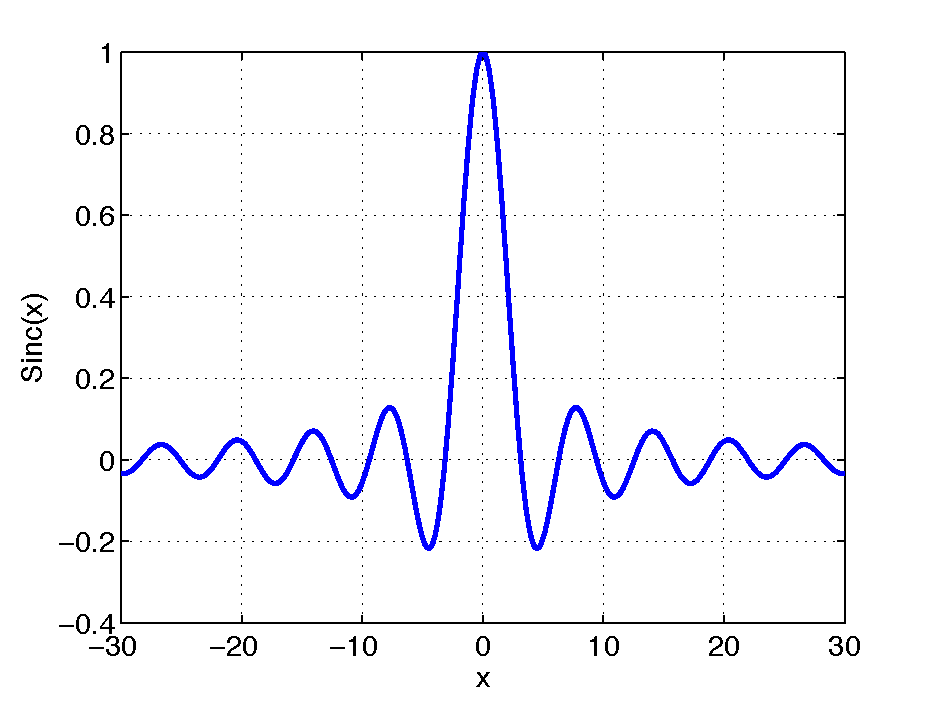
\includegraphics[width=.6\linewidth]{Figures/SincPlot}
%		\caption{Here goes the caption.}
%		\label{fig:Sinc}
%	\end{center}
%\end{figure}
%Figure~\ref{fig:Sinc} shows a shows a plot of the function $\sin(x)/x$. 
%
%If I need to make a simple diagram, I use powerpoint and select the drawing and save it as a pdf. For example, look at Figure~\ref{fig:MechaSys}.
%\begin{figure}[ht]
%	\begin{center}
%		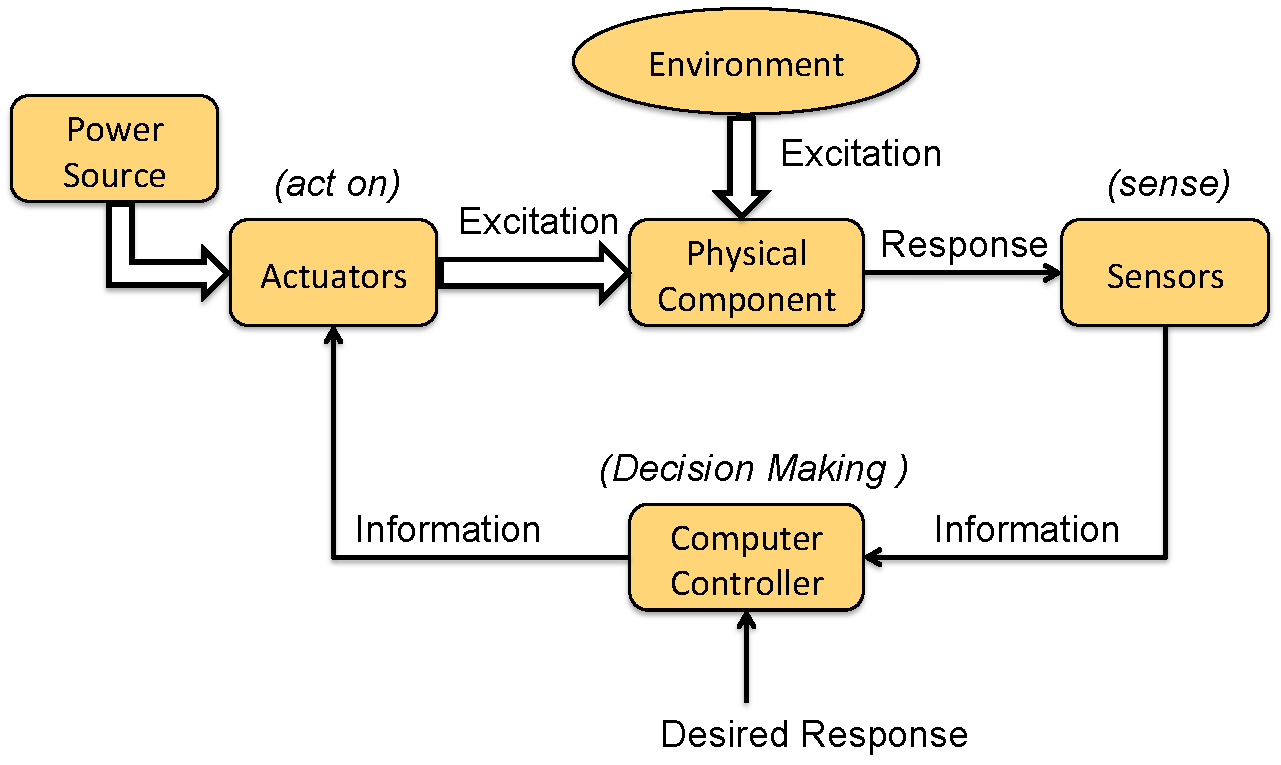
\includegraphics[width=.6\linewidth]{Figures/MechaSys}
%		\caption{Here goes the caption.}
%		\label{fig:MechaSys}
%	\end{center}
%\end{figure}
%
%
%To create lists use the environments \verb|itemize|, \verb|enumerate|, or \verb|description|
%
%The following is generated using \emph{itemize}
%\begin{itemize}
%	\item This is item 1 
%	\item This is item 2
%\end{itemize}
%%
%The following is generated using \emph{enumerate}
%\begin{enumerate}[1)]
%	\item This is item 1 
%	\begin{enumerate}[a)]
%		\item Subitem a
%		\item Subitem b
%		\begin{enumerate}[i)]
%			\item Subsubitem i
%			\item Subsubitem ii
%		\end{enumerate}
%	\end{enumerate}
%	\item This is item 2
%\end{enumerate}
%%
%The following is generated using \emph{description}
%\begin{description}
%	\item[foo)] This is item 1 
%	\item[bar)] This is item 2
%\end{description}
%
%
%
%To include a syntax-highlighted code listing, you can use the \emph{listings} package. The default options are specified by the \verb|\lstset| command. There are 3 main commands, all of which can include options to override the defaults:
%\begin{enumerate}
%	\item \verb|\lstinline|: Command for including code fragments inline with the text, as an alternative to \verb|\verb|. For example, we might describe function prototypes such as \lstinline[language=C,breaklines=true]|int main(int argc, char *argv[])|.
%	\item \verb|\begin{lstlisting}|,\ldots,\verb|\end{lstlisting}|: Environment for including a source code listing---embedded in the LaTeX source---in a box or floating environment. An example is shown in Listing~\ref{lst:sqrt}.
%	\item \verb|\lstinputlisting|: Command for including a source code listing---loaded from an external file---in a box or floating environment. This method is preferred over including the code source within the LaTeX file, since the code and its documentation can always be kept in sync. An example is shown in Listing~\ref{lst:matlabserial}.
%\end{enumerate}
%
%\begin{lstlisting}[
%language=C,
%float=h,
%numbers=none,
%xleftmargin=1cm,
%frame=none,
%caption={A winning entry from the 16th International Obfuscated C Code Contest, that computes the square root of its input.\label{lst:sqrt}}
%]
%#include <stdio.h>
%int l;int main(int o,char **O,
%int I){char c,*D=O[1];if(o>0){
%for(l=0;D[l              ];D[l
%++]-=10){D   [l++]-=120;D[l]-=
%110;while   (!main(0,O,l))D[l]
%+=   20;   putchar((D[l]+1032)
%/20   )   ;}putchar(10);}else{
%c=o+     (D[I]+82)%10-(I>l/2)*
%(D[I-l+I]+72)/10-9;D[I]+=I<0?0
%:!(o=main(c/10,O,I-1))*((c+999
%)%10-(D[I]+92)%10);}return o;}
%\end{lstlisting}
%
%\lstinputlisting[
%language=Matlab,
%float=h,
%numbers=left,
%xleftmargin=1cm,
%frame=shadowbox,
%caption={Matlab serial communication example.\label{lst:matlabserial}},
%morekeywords={try,catch}
%]{Code/serialtest.m}
%

\end{document}
